\documentclass[tikz, border=10pt]{standalone}

% Required packages
\usepackage[utf8]{inputenc}
\usepackage[T1]{fontenc}
\usepackage{lmodern} % For smooth fonts
\usepackage{tikz}

% TikZ libraries for advanced features
\usetikzlibrary{
    positioning,      % For placing nodes relative to each other
    arrows.meta,      % For modern arrow tips
    calc              % For coordinate calculations
}

\begin{document}
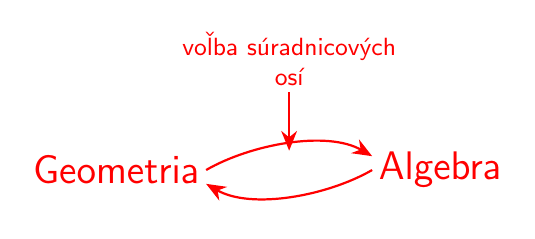
\begin{tikzpicture}[
    % Global style settings
    node distance=1.5em and 3em, % Default spacing for nodes
    red_style/.style={
        color=red, 
        thick
    },
    arrow_tip/.style={
        -{Stealth[length=2.5mm, width=2mm]}
    },
    text_style/.style={ % Style for the main labels "Geometria" and "Algebra" (not all caps)
        red_style,
        font=\sffamily\Large, % Use a larger sans-serif font
        inner sep=2pt
    },
    annotation_style/.style={ % Style for the annotation text
        red_style,
        font=\sffamily\small, % Smaller sans-serif font
        inner sep=2pt
    }
]
    % 1. Define the main text nodes (not all caps).
    \node[text_style] (geometria) {Geometria};
    \node[text_style, right=6em of geometria] (algebra) {Algebra};

    % 2. Place the annotation text node above the arrows.
    \node[annotation_style, above=2em of $(geometria.north east)!0.5!(algebra.north west)$, align=center] (annotation_text) {voľba súradnicových \\ osí};

    % 3. Draw the down arrow, ending slightly above the midpoint.
    \draw[red_style, arrow_tip] (annotation_text.south) to[out=-90, in=90] ($(geometria.east)!0.5!(algebra.west) + (0, 0.7em)$);

    % 4. Draw the two curved arrows between Geometria and Algebra, shifted vertically.
    % The 'out' and 'in' angles are also slightly adjusted to keep a good curve.
    % Upper arrow (Geometria to Algebra) - shifted up
    \draw[red_style, arrow_tip] (geometria.east) to[out=30, in=150, looseness=0.8] ($(algebra.west)+(0,0.5em)$);

    % Lower arrow (Algebra to Geometria) - shifted down
    \draw[red_style, arrow_tip] (algebra.west) to[out=-150, in=-30, looseness=0.8] ($(geometria.east)-(0,0.5em)$);

\end{tikzpicture}
\end{document}
